
\chapter{实验过程与分析}

\section{实验环境}
对于前面提出的基于图像的树木轻量化建模方法,本文做了大量实验验证了其可行性。
本文使用的拍摄工具是高分辨率安卓手机索尼LT26ii,该手机最高分辨率能达到4000x3000,
已经足够实验的需求。拍摄地点为同济大学嘉定校区以及某住宅小区。本文实验所使用计算机
操作系统平台为XUbuntu 12.04,CPU为双核Intel(R) Core(TM) i5-3230M @ 2.60GHz。显卡为
NVidia GeForce GT750M。 所有实验程序均使用C/C++语言完成,使用g++编译器进行编译,
同时使用OpenGL version 4.3图形硬件接口来完成可视化工作。

\section{实验结果与分析}
本文以三棵树的建模结果作为展示和分析的依据,其中第一棵树拍摄帧数为20帧,见图\ref{fig:sample1}。
第二棵树的拍摄帧数为12帧,见图

% sample 1
\begin{figure}
	\captionsetup[subfigure]{labelformat=empty}
	\subfloat[]{
	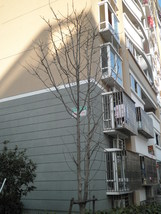
\includegraphics[height=2cm]{sample1_1.jpg}}
	\hspace{1mm}
	\subfloat[]{
	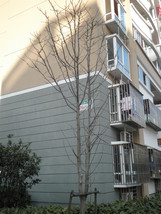
\includegraphics[height=2cm]{sample1_2.jpg}}
	\hspace{1mm}
	\subfloat[]{
	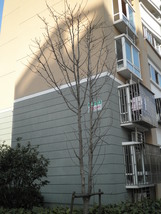
\includegraphics[height=2cm]{sample1_3.jpg}}
	\hspace{1mm}
	\subfloat[]{
	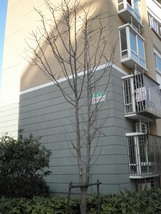
\includegraphics[height=2cm]{sample1_4.jpg}}
	\hspace{1mm}
	\subfloat[]{
	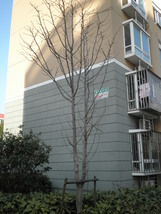
\includegraphics[height=2cm]{sample1_5.jpg}}
	\hspace{1mm}
	\subfloat[]{
	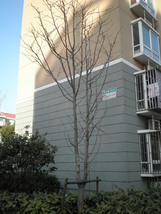
\includegraphics[height=2cm]{sample1_6.jpg}}
	\hspace{1mm}
	\subfloat[]{
	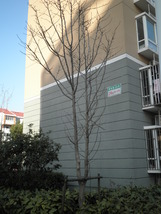
\includegraphics[height=2cm]{sample1_7.jpg}}
	\hspace{1mm}
	\subfloat[]{
	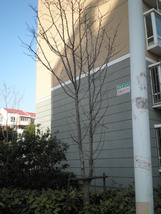
\includegraphics[height=2cm]{sample1_8.jpg}}
	\hspace{1mm}
	\subfloat[]{
	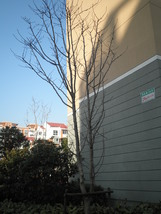
\includegraphics[height=2cm]{sample1_9.jpg}}
	\hspace{1mm}
	\subfloat[]{
	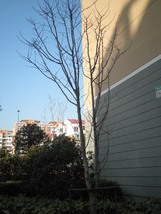
\includegraphics[height=2cm]{sample1_10.jpg}}
	\hspace{1mm}
	\subfloat[]{
	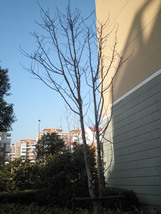
\includegraphics[height=2cm]{sample1_11.jpg}}
	\hspace{1mm}
	\subfloat[]{
	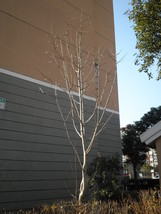
\includegraphics[height=2cm]{sample1_12.jpg}}
	\hspace{1mm}
	\subfloat[]{
	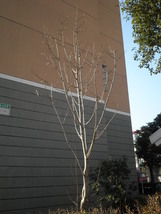
\includegraphics[height=2cm]{sample1_13.jpg}}
	\hspace{1mm}
	\subfloat[]{
	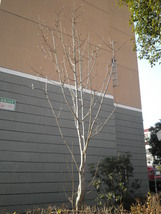
\includegraphics[height=2cm]{sample1_14.jpg}}
	\hspace{1mm}
	\subfloat[]{
	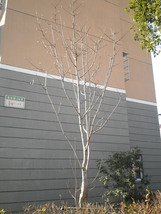
\includegraphics[height=2cm]{sample1_15.jpg}}
	\hspace{1mm}
	\subfloat[]{
	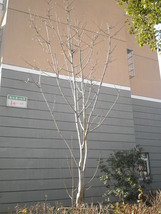
\includegraphics[height=2cm]{sample1_16.jpg}}
	\hspace{1mm}
	\subfloat[]{
	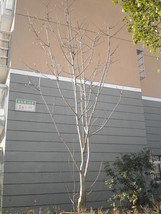
\includegraphics[height=2cm]{sample1_17.jpg}}
	\hspace{1mm}
	\subfloat[]{
	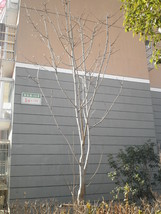
\includegraphics[height=2cm]{sample1_18.jpg}}
	\hspace{1mm}
	\subfloat[]{
	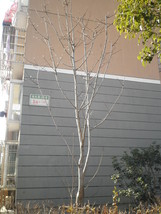
\includegraphics[height=2cm]{sample1_19.jpg}}
	\hspace{1mm}
	\subfloat[]{
	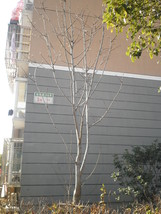
\includegraphics[height=2cm]{sample1_20.jpg}}
	\hspace{1mm}
	\caption{树木1图像序列,帧数为20帧,拍摄地点为某住宅小区}
	\label{fig:sample1}
\end{figure}

% sample 2
\begin{figure}
	\captionsetup[subfigure]{labelformat=empty}
	\subfloat[]{
	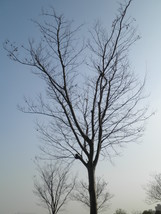
\includegraphics[height=2cm]{sample2_1.jpg}}
	\hspace{1mm}
	\subfloat[]{
	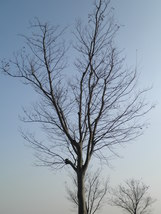
\includegraphics[height=2cm]{sample2_2.jpg}}
	\hspace{1mm}
	\subfloat[]{
	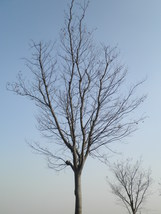
\includegraphics[height=2cm]{sample2_3.jpg}}
	\hspace{1mm}
	\subfloat[]{
	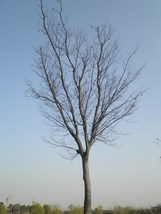
\includegraphics[height=2cm]{sample2_4.jpg}}
	\hspace{1mm}
	\subfloat[]{
	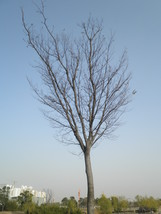
\includegraphics[height=2cm]{sample2_5.jpg}}
	\hspace{1mm}
	\subfloat[]{
	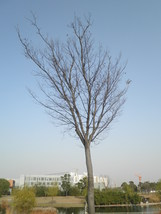
\includegraphics[height=2cm]{sample2_6.jpg}}
	\hspace{1mm}
	\subfloat[]{
	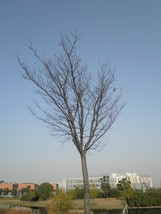
\includegraphics[height=2cm]{sample2_7.jpg}}
	\hspace{1mm}
	\subfloat[]{
	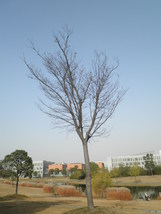
\includegraphics[height=2cm]{sample2_8.jpg}}
	\hspace{1mm}
	\subfloat[]{
	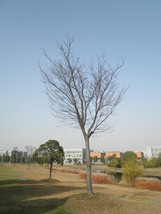
\includegraphics[height=2cm]{sample2_9.jpg}}
	\hspace{1mm}
	\subfloat[]{
	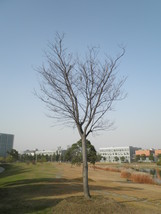
\includegraphics[height=2cm]{sample2_10.jpg}}
	\hspace{1mm}
	\subfloat[]{
	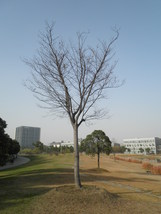
\includegraphics[height=2cm]{sample2_11.jpg}}
	\hspace{1mm}
	\subfloat[]{
	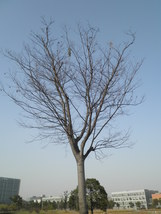
\includegraphics[height=2cm]{sample2_12.jpg}}
	\caption{树木2图像序列,帧数为12帧,拍摄地点为同济大学嘉定校区}
	\label{fig:sample2}
\end{figure}
